\documentclass[12pt, twoside]{article}
\usepackage[utf8]{inputenc}
\usepackage[english]{babel}

\usepackage{amsthm}
\usepackage{a4wide}
\usepackage{graphicx}
\usepackage{caption}
\usepackage{subcaption}
\usepackage{amssymb}
\usepackage{amsmath}
\usepackage{mathrsfs}
\usepackage{euscript}
\usepackage{graphicx}
\usepackage{caption}
\usepackage{color}
\usepackage{bm}
\usepackage{tabularx}
\usepackage{adjustbox}
\usepackage[toc,page]{appendix}
\usepackage{comment}
\usepackage{rotating}

\DeclareMathOperator*{\argmax}{arg\,max}
\DeclareMathOperator*{\argmin}{arg\,min}
\newtheorem{definition}{Definition}[section]
\numberwithin{equation}{section}
\newcommand*{\No}{No.}

\begin{document}


\title{\bf Analysis of the properties of probabilistic models in learning problems with an expert}
\date{}
\author{}
\maketitle



\begin{center}
\bf
A.\,I. Bazarova\footnote{Moscow Institute of Physics and Technology, bazarova.ai@phystech.edu}, 
A.\,V.~Graboviy\footnote{Moscow Institute of Physics and Technology, grabovoy.av@phystech.edu}, 
V.\,V.~Strijov\footnote{Moscow Institute of Physics and Technology, strijov@phystech.edu}

\end{center}
{\centering\begin{quote}
\textbf{Abstract:} This paper is devoted to the construction of interpretable models in machine learning. 
It solves the problem of approximating a given set of figures on a contour image.
Assumptions are introduced that the figures are curves of the second order.
When approximating figures, information about the type, location and form of curves, as well as the set of their possible transformations, is used.
Such information is called \textit{expert}, and the machine learning method based on expert information is called \textit {expert learning}.
It is assumed that the set of shapes is approximated by a set of \textit {local models}.
Each local model, based on expert information, approximates one shape in the contour image.
To build models, it is proposed to map second-order curves into a feature space where each local model is a linear model.
Thus, higher-order curves are recognized using the composition of linear models.
As an applied problem, the problem of approximating the iris of the eye on a contour image is considered.
    

    
\smallskip
\textbf{Keywords}: mixture of experts, expert learning, linear models, interpretabe models
\smallskip
%\textbf{DOI}: 00.00000/00000000000000
\end{quote}
}

\section {Introduction}
Interpretable model building in machine learning~\cite{Ribeiro2016} is one of the key challenges.
Modern solutions of the image classification problem based on deep learning networks ResNet, VGG, Intercept~\cite{Kaiming2015} are poorly interpreted models.
The papers~\cite{Han2020, Xingjun2019, Akhtar2018} show that deep learning networks are sensitive even to small noise in the data, which is due to their uninterpretability.

In this paper, we propose a \textit {training with an expert} method.
This method assumes the use of subject knowledge of experts to improve the quality of approximation, as well as to obtain interpretable machine learning models.
The subject knowledge of experts about the sample will be called~\textit {expert information}.
It is assumed that the use of expert information allows the sample to be approximated by simple interpretable models, such as linear models. Machine learning methods that take expert knowledge into account when building models are called~\textit {expert learning}.

This paper solves the problem of approximating second-order curves on a contour image. Second-order curves are selected for analysis, since they are easily described by linear models. In this case, these figures need to be restored in such applied problems as the problem of recognizing the iris of the eye~\cite{Matveev2010, Matveev2014, Bowyer2010}, the problem of describing the particle track in the hadron collider~\cite{Dalila2018}. Expert information about a second-order curve allows you to map points on a plane into a new feature description, where each curve is approximated by one linear model. A model that approximates one curve is called a \textit {local model}. To approximate the entire contour image, it is required to approximate several second-order curves using several local models. In this paper, the following restrictions on images are introduced:
\begin{enumerate}
	\item[1)] the image consists only of second-order curves;
	\item[2)] the image is approximated by a small number of second-order curves;
	\item[3)] the number and type of curves in the image is known.
\end{enumerate}

\begin{figure}[h!]
     \centering
     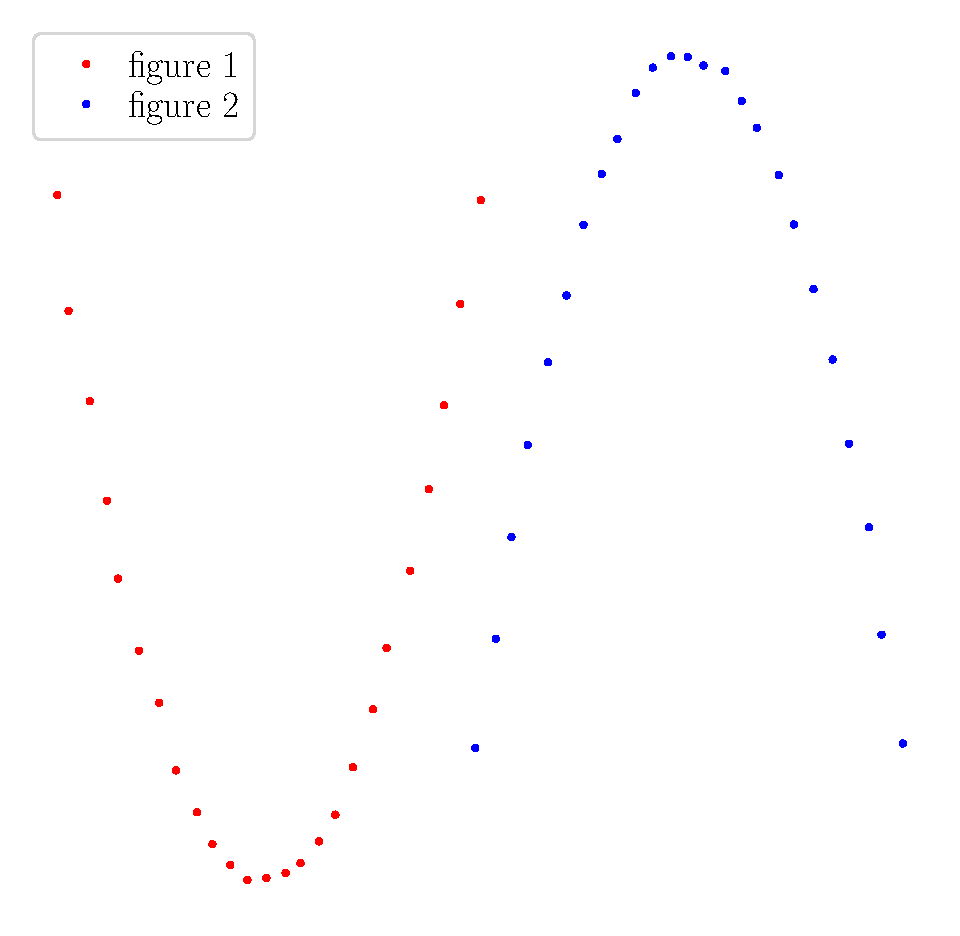
\includegraphics[width=\textwidth]{figures/explanation}
\caption {Example: a) expert information of the first expert; b) baseline data; c) expert information of the second expert.}
    \label{intro:fig2}
\end{figure}

Figure~\ref{intro:fig2} shows an example of second-order curves, as well as expert information on curves. Figure~\ref{intro:fig2} a shows the expert information of the first expert. Using this information, the first curve is fitted with a linear model and the second curve is noise. Figure~\ref{intro:fig2} b shows the expert information of the second expert. Using this information, the second curve is fitted with a linear model and the first curve is noise.

When approximating several curves on one contour image, a multi-model is built. An example of multi-models is a random forest~\cite{Ishwaran2012}, tree boosting~\cite{Tianqi2016}, a mixture of experts~\cite{Yuksel2012}. In this paper, a mixture of experts is considered as a multi-model. Expert mixture is a multi-model that linearly weights local models that approximate a portion of the sample. The values of the weighting coefficients depend on the object for which the prediction is made. To solve the problem of a mixture of experts, a variational EM-algorithm~\cite{Dempster1977, bishop2006, Peng1996} is used. The mixture of experts has many uses in a number of applications. In the paper~\cite{Estabrooks2001}, the text classification problem is solved. In the paper~\cite{Cheung1995, Weigend2000, Cao2003, Mossavat2010, Sminchisescu2007, Tuerk2001, Yumlu2003}, a mixture of experts is used to predict time series for speech recognition, daily human activity, and prediction of the value of securities. In the paper~\cite{Ebrahimpour2009}, a mixture of experts was considered to solve the problem of recognizing handwritten numbers in images.

As an example, the problem of approximation of the iris image is considered. Figure~\ref{intro:fig1:real} shows an example of the image that needs to be approximated. In this paper, we consider a processed image, which is given in outline form, an example of such an image is shown in Figure~\ref{intro:fig1:outer}. Figure~\ref{intro:fig1:outer} shows two local circle models that approximate the iris of the eye. Circumferences are a simple example of a second order curve.

\begin{figure}[h!]
     \centering
     \begin{subfigure}[b]{0.3\textwidth}
         \centering
         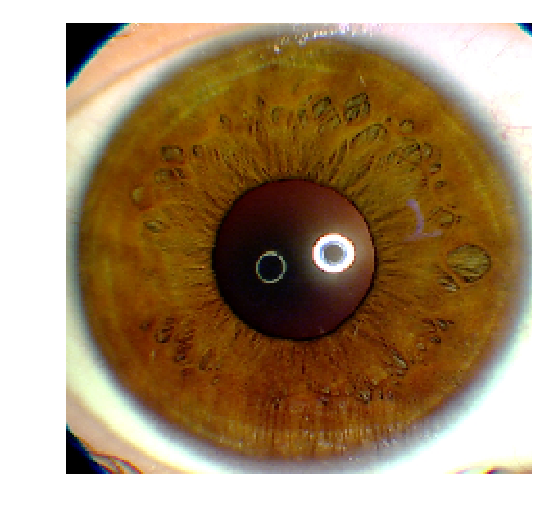
\includegraphics[width=\textwidth]{figures/real_image}
         \caption{}
         \label{intro:fig1:real}
     \end{subfigure}
     \begin{subfigure}[b]{0.3\textwidth}
         \centering
         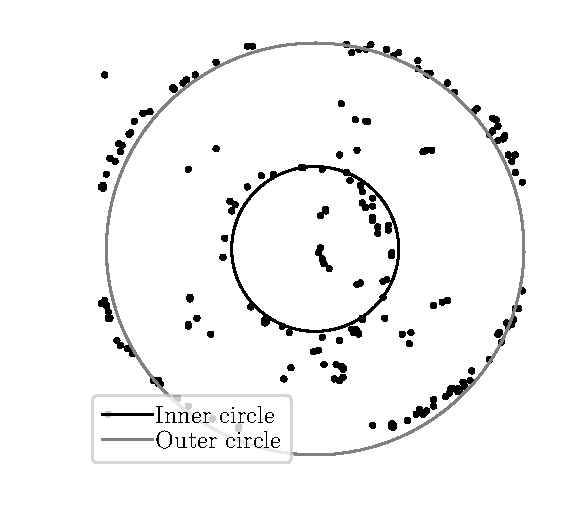
\includegraphics[width=\textwidth]{figures/outline_image}
         \caption{}
         \label{intro:fig1:outer}
     \end{subfigure}
\caption{An example of the image of the iris of the eye and its outline representation: a) the image of the iris of the eye; b) contour image of the iris and approximating the given image of the circumferences.}    \label{intro:fig1}
\end{figure}

For the problem of approximating the iris of the eye, the following expert information is used: the iris of the eye is approximated by two concentric circumferences. Expert information is used to construct a feature description of plane points, as well as to build an optimization function. The part of the error function for optimization that uses expert information is called a regularizer. Thus, the information that the image of the circumferences is specified by the feature description, and the information that the concentric circumferences are specified using a special regularizer.

In a computational experiment, the quality of the approximation of the contour image is analyzed depending on the specified expert information and on the noise level in the synthetically generated data. The analysis of the quality of the approximation of the iris is carried out, depending on the amount of expert information that was used to build the model. Note that each approximated image is a separate set of points that need to be approximated.

\section{Statement of the problem of finding the parameters of the second-order curves in the image}
Binary image is set:
$$ \mathbf{M} \in \{0, 1 \}^{m_1\times m_2},$$
where 1 corresponds to the black point of the image, and 0 corresponds to the white point of the background.
From the image $\mathbf {M} $, a sample$ \mathbf{C}$ is constructed, the elements of which are the coordinates $(x_i, y_i)$ of black points: $$\mathbf {C} \in \mathbb {R}^{N \times 2}. $$
The expert assumes that the image consists of a second-order curve~$\Omega$.
Let for a set of points $\mathbf {C} \in \mathbb {R}^{N \times 2} $ that form a curve $\Omega, $ expert information about the figure $E(\Omega) $is given.
The set $E (\Omega)$ consists of the shape $\Omega$ expected by the expert and the set of its admissible transformations. Based on the expert description, let us introduce mappings into a new problem for approximation:
\begin{equation}\label{eq1}
	K_{x}\bigl(E(\Omega)\bigr): \mathbb{R}^{2} \rightarrow \mathbb{R}^{n}, \quad K_{y}\bigl(E(\Omega)\bigr): \mathbb{R}^{2} \rightarrow \mathbb{R},
\end{equation} 
where~$K_{x}$ mapping objects to the attribute description of objects,~$n$is the number of features, and~$K_ {y}$ is a mapping to a target variable for an object. Applying the mappings~$K_ {x}, K_{y}$for the sample~$\mathbf {C}$ element by element we obtain:
\begin{equation}
\label{eq2}
	K_{x}\bigl(E(\Omega\bigr), \mathbf{c}) = \mathbf{x}, \quad  K_{y}\bigl(E(\Omega), \mathbf{c}\bigr) = y,
\end{equation}
where~$\mathbf{c} = (x_i, y_i)$ is a sample point $\mathbf{C}$.

Applying the mappings \eqref{eq2} to the original set of points $\mathbf {C} $, we obtain the sample
\begin{equation}
\label{eq4}
    \mathfrak{D} = \{(\mathbf{x}, y) \; | \; \forall \mathbf{c} \in \mathbf{C} \; \mathbf{x} = K_x(\mathbf{c}), \; y = K_y(\mathbf{c}) \}.
\end{equation}

We get that the original problem of curve approximation~$\Omega$ is reduced to approximation of the sample~$\mathfrak {D}$. In this paper, it is assumed that the sample~$\mathfrak {D}$ is approximated by a linear model:
\begin{equation}
	g(\mathbf{x}, \mathbf{w}) = \mathbf{x}^\mathsf{T} \mathbf{w},
\end{equation} 
where~$\mathbf{w}$ vector, the parameter to be found.

To find the optimal vector of parameters~$\hat {\mathbf {w}}$, it is required to solve the following optimization problem:
\begin{equation}
	\hat{\mathbf{w}} = \arg\min_{\mathbf{w}\in\mathbb{R}^n} \sum_{\left(\mathbf{x}, y\right) \in \mathfrak{D}}\|g(\mathbf{x}, \mathbf{w}) - y \|_2^2.
\end{equation} 

Thus, the problem of approximating the original curve~$\Omega$ is reduced to solving the problem of linear regression, i.e. finding the components of the vector $\hat{\mathbf {w}}$ connecting the resulting $\mathbf {x}$ and $y$.

In the case when on the image $K$ the second-order curves  $\Omega_1, \dots, \Omega_K$, for each of which there is expert information $E_k = E (\Omega_k), \, k \in \{1, \dots , K\}$, the problem of constructing a multi-model called a mixture of $K$ experts is posed.
\begin{definition}
We call the multimodel $ f $ a mixture of K experts
\begin{equation}
	f = \sum\limits_{k = 1}^{K}\pi_k(\mathbf{x}, \mathbf{V})g_k(\mathbf{w}_k),  \quad \pi_k(\mathbf{x}, \mathbf{V}): \mathbb{R}^{n\times |\mathbf{V}|} \rightarrow [0, \, 1], \quad \sum\limits_{k = 1}^{K}\pi_k(\mathbf{x}, \mathbf{V}) = 1, 
\end{equation}
where $g_k$ is a local model called by the expert, $\mathbf{x}$is an attribute description of an object, $\pi_k$is a gateway function, the vector $\mathbf{w}_k$ are local model parameters, the vector $\mathbf{V}$ are gateway function parameters. In this paper, $g_k$ is a linear model.
\end{definition}

For each second-order curve, mappings (\ref{eq1}) are given. For convenience, we introduce the following notation: $K_x^k\bigr(\mathbf{c}\bigr) = K_x\bigr(\Omega_k, \mathbf{c}\bigr)$ and $K_y^k\bigr(\mathbf{c}\bigr) = K_y\bigr(\Omega_k, \mathbf{c}\bigr)$. Then, using local linear models, we construct a universal multi-model describing the curves $\Omega_1, \dots, \Omega_K$ on the image $\mathbf{M}$:
\begin{equation}
\label{5}
	f = \sum\limits_{\mathbf{c} \in \mathbf{C}} \sum_{k = 1}^{K} \pi_k(\mathbf{c}, \mathbf{V})g_k(K^k_{x}\bigl(\mathbf{c}), \mathbf{w}_k), 
\end{equation}
where $\pi_k$ is the  gateway function. In this paper, we consider a simple case, where~$\mathbf{x}=K^1_{x}\bigl(\mathbf{c})=\cdots=K^K_{x}\bigl(\mathbf{c}),$ then the expression~\eqref{5} is rewritten in the following simple form:
\begin{equation}
\label{5_1}
	f = \sum\limits_{\mathbf{c} \in \mathbf{C}} \sum_{k = 1}^{K} \pi_k(\mathbf{x}, \mathbf{V})g_k(\mathbf{x}, \mathbf{w}_k), 
\end{equation}
where the gateway function $\pi_k$ has the following form:
\begin{equation}
\label{6}
	\pi_k(\mathbf{x}, \mathbf{V}): \mathbb{R}^{n\times |\mathbf{V}|} \rightarrow [0, \, 1], \; \; \; \; \sum\limits_{k = 1}^{K}\pi_k(\mathbf{x}, \mathbf{V}) = 1,
\end{equation}
where $\mathbf{V}$ are the gateway function parameters, and $g_k$ is a local model.
    
In this paper
\begin{equation}
    \boldsymbol{\pi}(\mathbf{x}, \mathbf{V}) = \text{softmax}\bigl(\mathbf{V}_1^{\mathsf{T}}\boldsymbol{\sigma}(\mathbf{V}_2^{\mathsf{T}}\mathbf{x}) \bigr),
\end{equation}
where $\mathbf{V} = \{ \mathbf{V}_1, \, \mathbf{V}_2\}$ are the gateway function parameters,
$\mathbf{V}_1 \in \mathbb{R}^{p \times k}, \, \mathbf{V}_2 \in \mathbb{R}^{n \times p}$. 

To find the optimal parameters of the multi-model, it is necessary to solve the following optimization problem:
\begin{equation}\label{9}
\mathcal{L} = \sum\limits_{(\mathbf{x}, y) \in \mathfrak{D}} \sum\limits_{k = 1}^{K} \pi_k(\mathbf{x}, \mathbf{V})(y - \mathbf{w}_k^{\mathsf{T}}\mathbf{x})^2 + R\bigl(\mathbf{V}, \mathbf{W}, E(\Omega)\bigr) \rightarrow \min_{\mathbf{V}, \mathbf{W}},
\end{equation}
where $\mathbf{W} = [\mathbf{w}_1, \dots, \mathbf{w}_k]$ are  parameters of local models, $R\bigl(\mathbf{V}, \mathbf{W}, E(\Omega)\bigr)$ is regularization parameters, based on expert information.

\section{Building an attribute description of figures }
\paragraph{ Unified space for second-order curves.} An arbitrary second-order curve, the main axis of which is not parallel to the ordinate axis, is given by the following expression:
\[
\label{st:coef}
x^2 = B'xy+C'y^2+D'x+E'y+F',
\]
where the coefficients $B ', C'$ are subject to restrictions that depend on the type of the curve. The expression~\eqref{eq2} takes the following form:
\[
\label{st:K_map}
K_x\bigr(\mathbf{c}_i\bigr)=\left[x_iy_i, y_i^2, x_i, y_i, 1\right], \quad K_y\bigr(\mathbf{c}_i\bigr)=x_i^2,
\]
whence we obtain the linear regression problem for recovering the parameters~$ B ', C', D ', E', F '$ from the selected sample.

\paragraph{ Circumference.} As a special case of a second-order curve, we consider the circumference.
Let $(x_0, y_0)$ be the center of the circumference to be found on the binary image $\mathbf {M} $, and $r$ be its radius.
The sample elements $(x_i, y_i) \in \mathbf {C}$ are the locus of points, which is approximated by the equation of the circumference:
\begin{equation}
(x_i - x_0)^2 + (y_i - y_0)^2 = r^2.
\end{equation}
Expanding the brackets, we get:
\begin{equation}(2x_0)\cdot x_i + (2y_0)\cdot y_i + (r^2 - x_0^2 - y_0^2)\cdot 1 = x_i^2 + y_i^2 . 
\end{equation}
Then the presentations (\ref{eq2}) take the following form:
\begin{equation}
\label{10}
K_{x}(\mathbf{c}_i) = [x_i, \, y_i, \, 1] = \mathbf{x}, \,  K_{y}(\mathbf{c}_i) = x_i^2+y_i^2 = y.
\end{equation} 
Assign the linear regression problem \eqref{eq4}.
Vector components $\mathbf{w} = [w_0, \, w_1, \, w_2]^\mathsf{T}$, binding $\mathbf{x}$ and $y$, restore the parameters of the circumference: \begin{equation} x_0 = \frac{w_0}{2}, \; y_0 = \frac{w_1}{2}, \; r = \sqrt{w_3 + x_0^2 + y_0 ^2}.\end{equation}

\section{Composition of figures }
To construct a composition of figures, we will use the expression~\eqref{9}, which takes the following form:
\begin{equation} 
\label{statment:optim:task}
\begin{aligned}
\mathcal{L} = \sum\limits_{\mathbf{c} \in \mathbf{C}} \sum\limits_{k = 1}^{K} \pi_k(\mathbf{c}, \mathbf{V})\left(K^{k}_y\bigr(\mathbf{c}\bigr) - \mathbf{w}_k^{\mathsf{T}}K^{k}_x\bigr(\mathbf{c}\bigr)\right)^2 + R\bigl(\mathbf{V}, \mathbf{W}, E(\Omega)\bigr) \rightarrow \min_{\mathbf{V}, \mathbf{W}},
\end{aligned}
\end{equation} 
where~$K^{k}_x, K^{k}_y$ expert representation of the~$k$-th expert. Assuming that all curves in the image are described by one attribute description $\mathbf {x} =K^{1}_x\bigr(\mathbf{c}\bigr)=\cdots=K^{K}_x\bigr(\mathbf{c}\bigr), x= K^{1}_y\bigr(\mathbf{c}\bigr)=\cdots=K^{K}_y\bigr(\mathbf{c}\bigr),$ we get the following optimization problem:
\begin{equation} 
\label{statment:optim:task:simp}
\begin{aligned}
\mathcal{L} = \sum\limits_{\left(\mathbf{x}, y\right) \in \mathfrak{D}} \sum\limits_{k = 1}^{K} \pi_k(\mathbf{x}, \mathbf{V})\left(y - \mathbf{w}_k^{\mathsf{T}}\mathbf{x}\right)^2 + R\bigl(\mathbf{V}, \mathbf{W}, E(\Omega)\bigr) \rightarrow \min_{\mathbf{V}, \mathbf{W}},
\end{aligned}
\end{equation} 

As a regularizer~$R$, additional restrictions on the vectors of model parameters are considered. To solve the optimization problem~\eqref{statment:optim:task:simp} it is proposed to use the EM-algorithm.

\section{ Computing experiment }
A computational experiment was carried out to analyze the quality of models of second-order curves in the image. The experiment is divided into several parts. The first part is an experiment with several circumferences in the image. The second part analyzes the convergence of the method depending on the noise level in the data and on the specified expert information. In the third part, an experiment is conducted to approximate the iris of the eye.

\subsection{ Experiment with circumstances }
\begin{figure}[h!]
\begin{minipage}{.32\textwidth}
      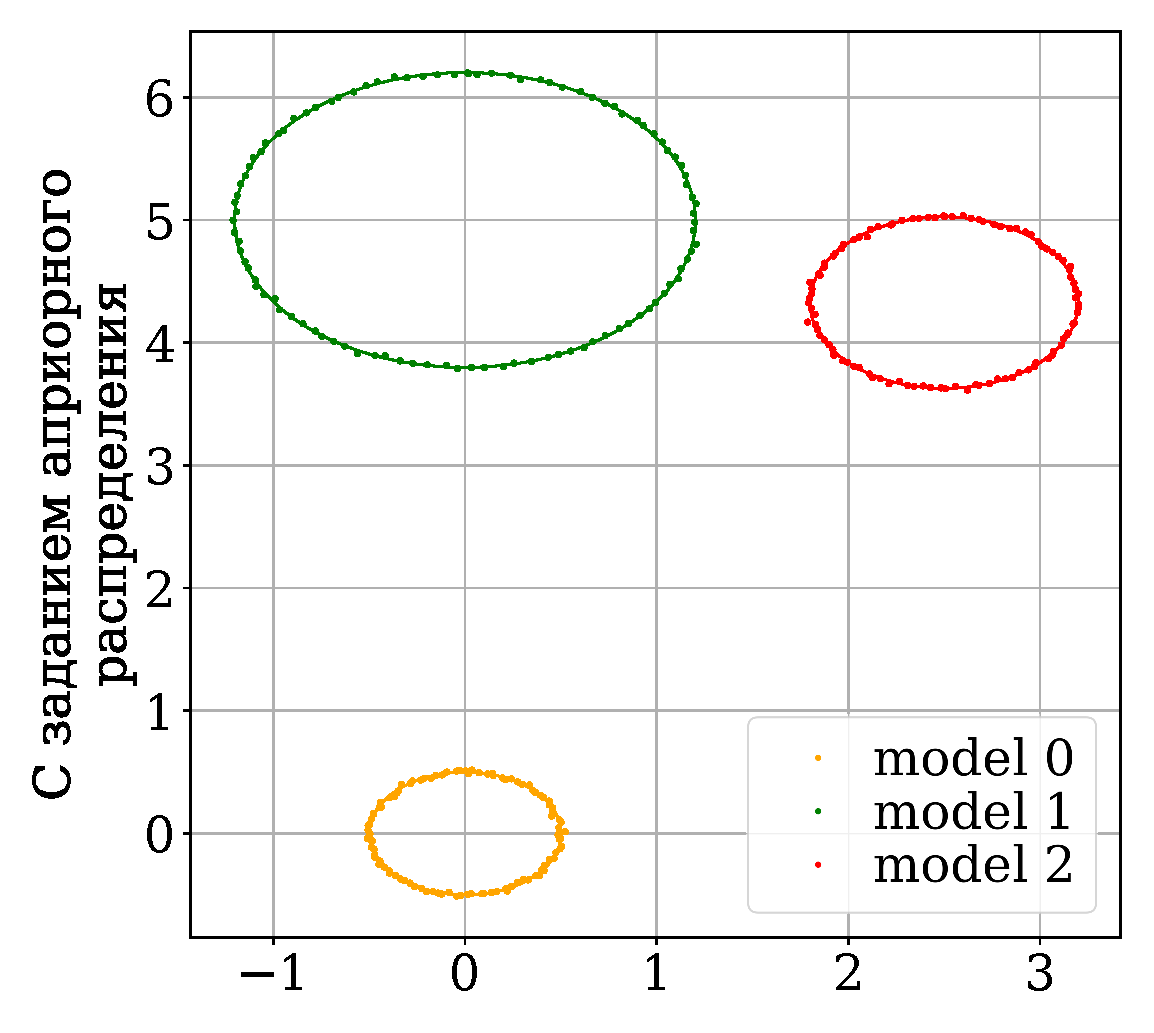
\includegraphics[width =  \textwidth]{figures/910.eps}
\end{minipage}
\begin{minipage}{.32\textwidth}
\hspace{0.3mm}
      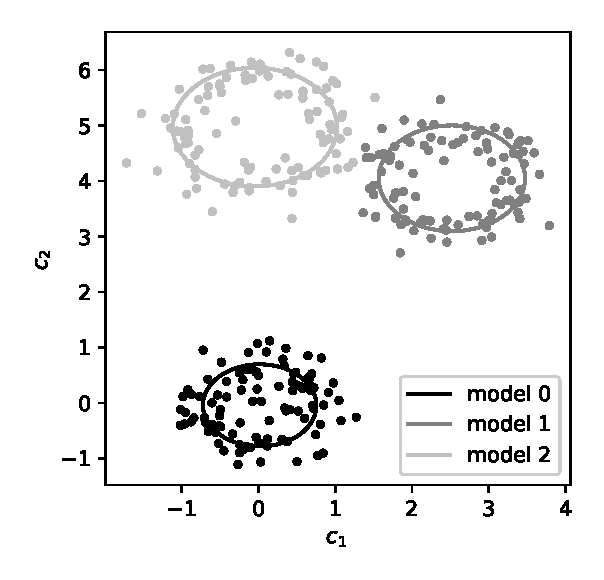
\includegraphics[width =  0.89\textwidth]{figures/901.eps}
\end{minipage}
\begin{minipage}{.32\textwidth}
\vspace{-3mm}
\hspace{-8.5mm}
      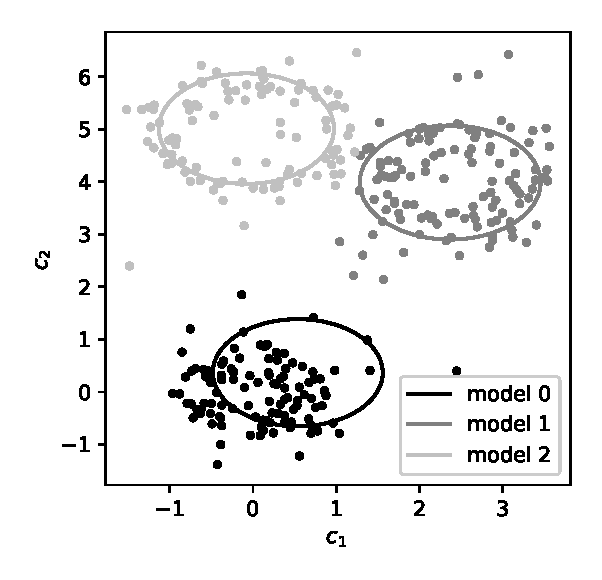
\includegraphics[width =  1.07\textwidth]{figures/902.eps}
\end{minipage}
\begin{minipage}{.32\textwidth}
      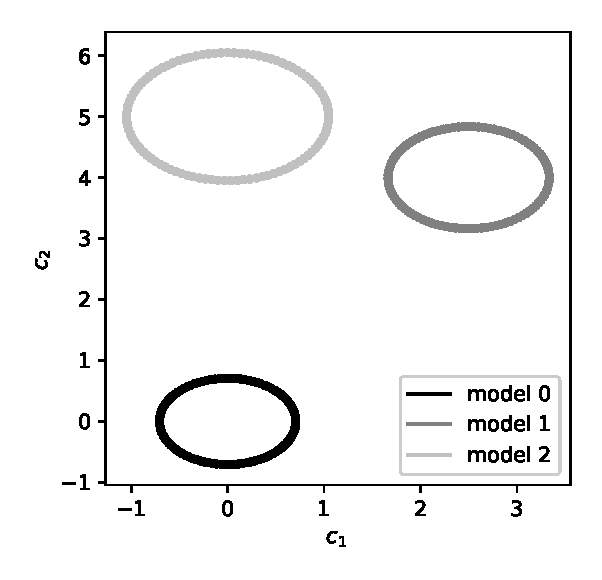
\includegraphics[width =  \textwidth]{figures/900.eps}
\end{minipage}
\begin{minipage}{.32\textwidth}
\hspace{2mm}
      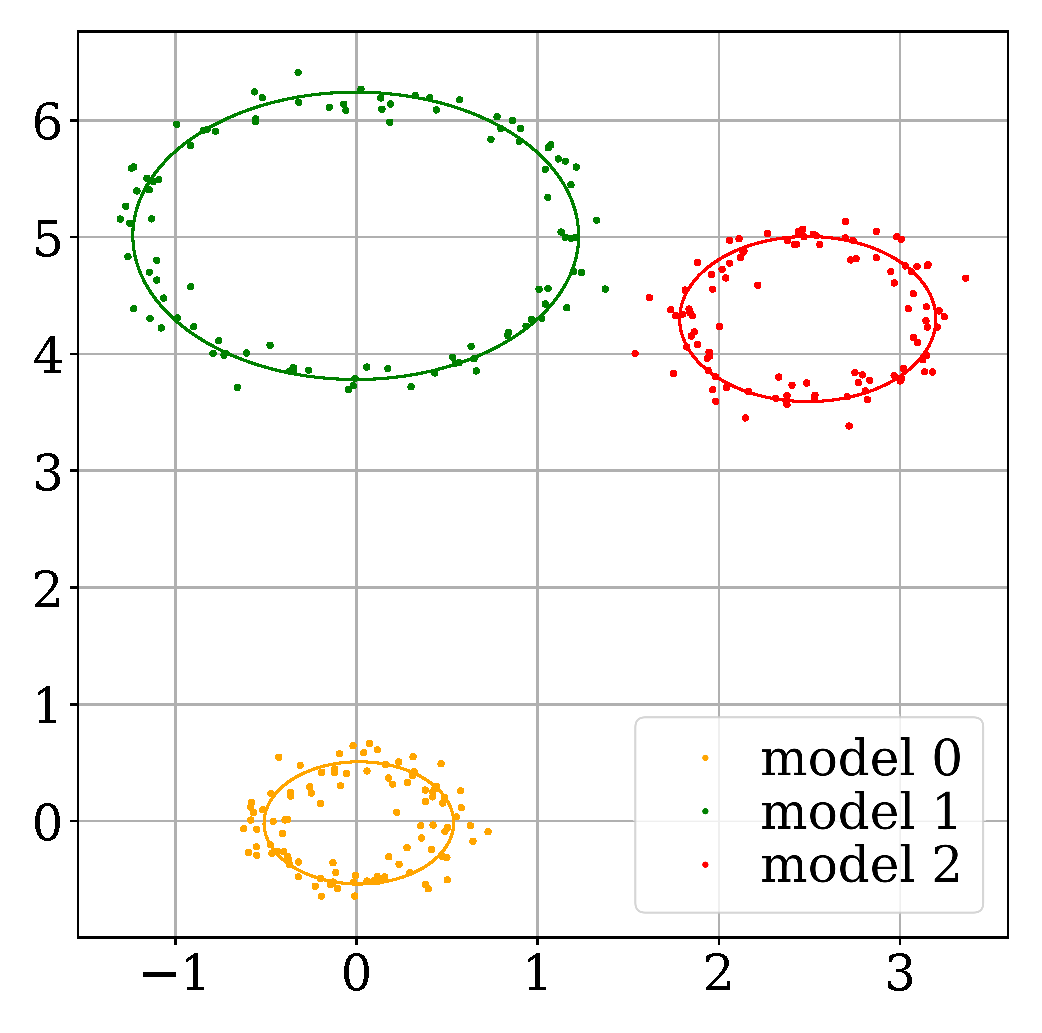
\includegraphics[width =  0.9\textwidth]{figures/911.eps}
\end{minipage}
\begin{minipage}{.32\textwidth}
\hspace{-2.3mm}
      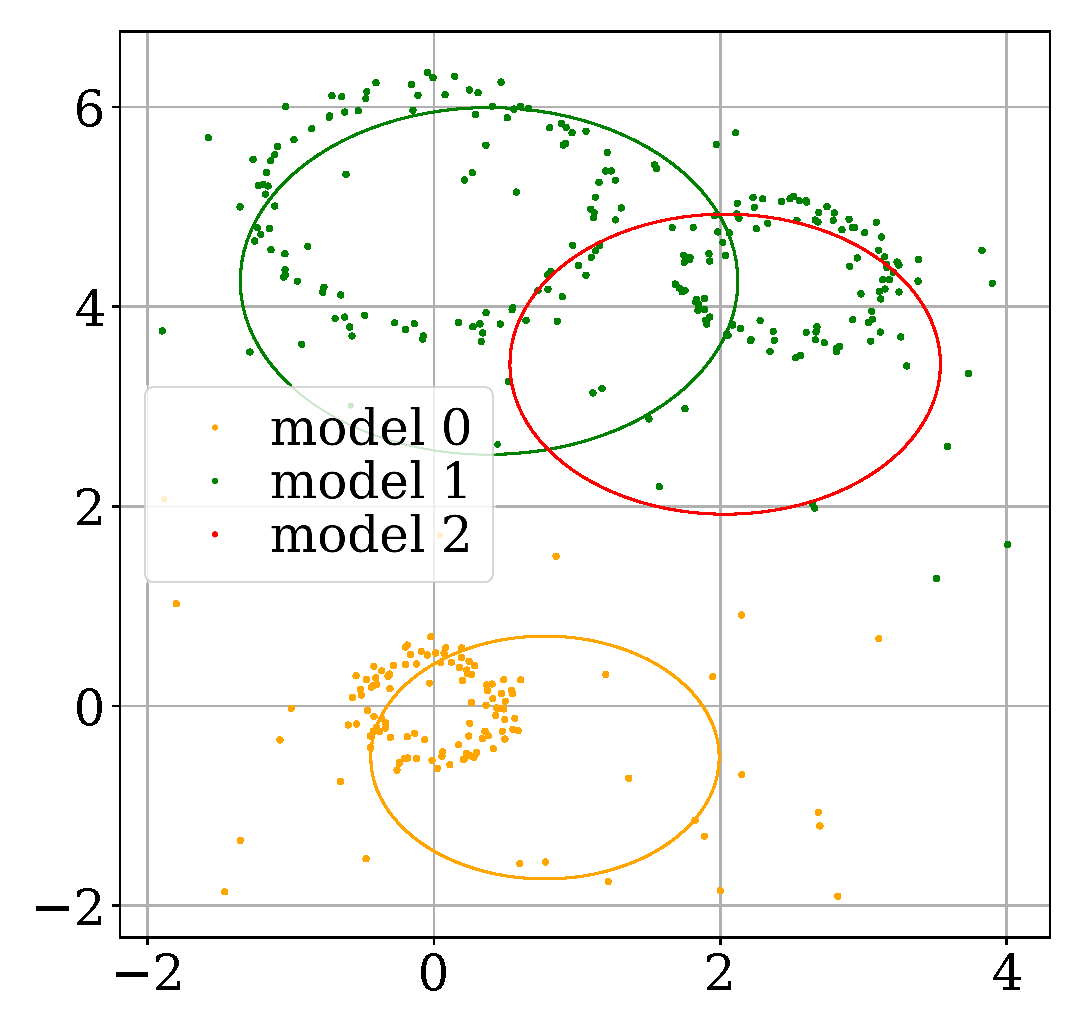
\includegraphics[width =  0.935\textwidth]{figures/912.eps}
\end{minipage}
\caption{Multi-model depending on different prior assumptions and noise level. From top to bottom: plotting with a priori distribution; without specifying the prior distribution. From left to right: circumferences without noise; noise in the radius of the circle; noise in the radius of a circle as well as arbitrary points throughout the image.}
\label{ce:fig3}
\end{figure}

\begin{figure}[h]
\begin{minipage}{.32\textwidth}
\hspace{-3mm}
      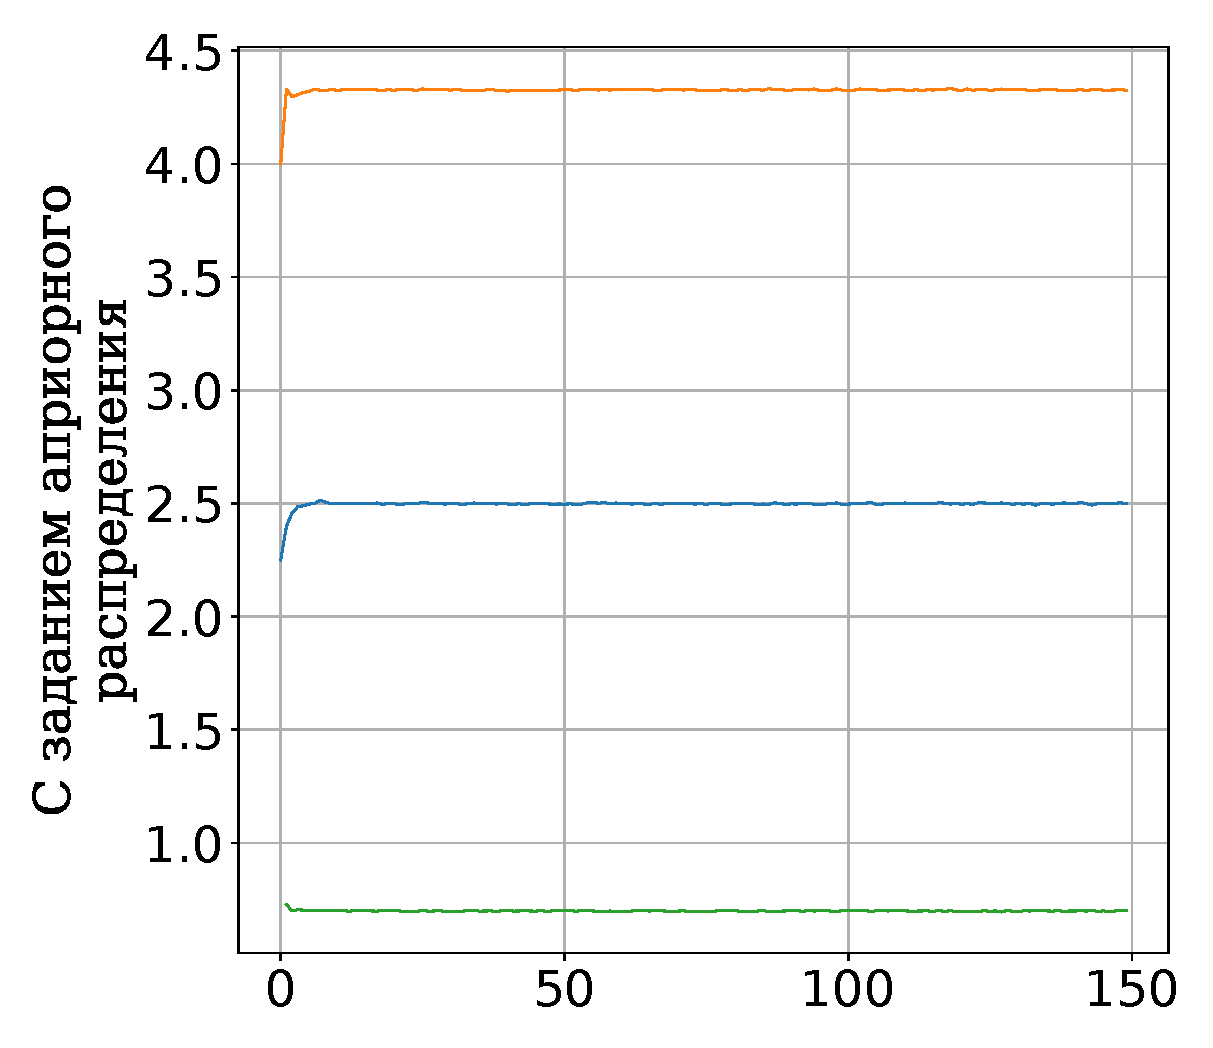
\includegraphics[width = 1.05\textwidth]{figures/910noise.eps}
\end{minipage}
\begin{minipage}{.32\textwidth}
\vspace{2pt}
\hspace{-2.1mm}
      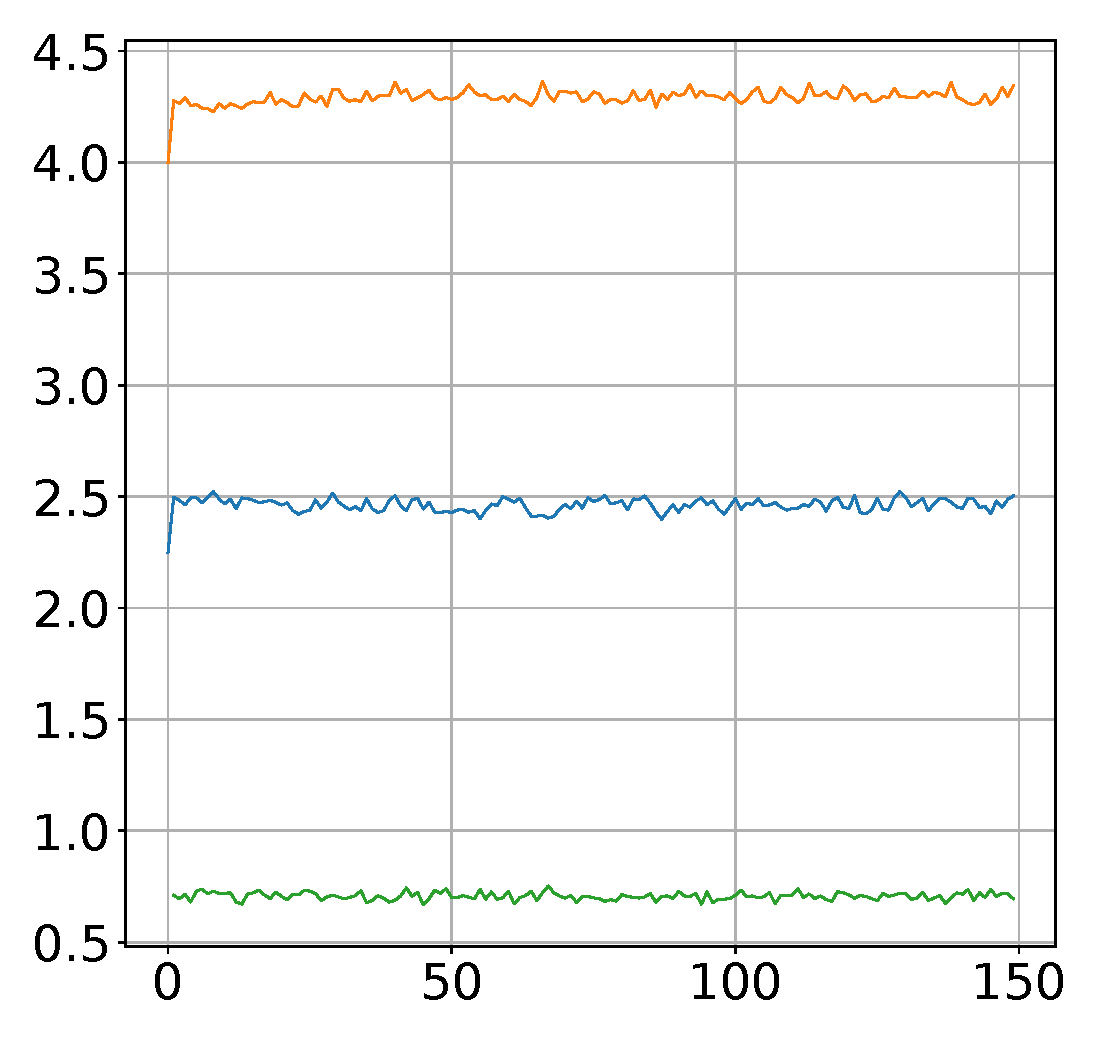
\includegraphics[width = 0.95\textwidth]{figures/911noise.eps}
\end{minipage}
\begin{minipage}{.32\textwidth}
\vspace{2pt}
\hspace{-6.3mm}
      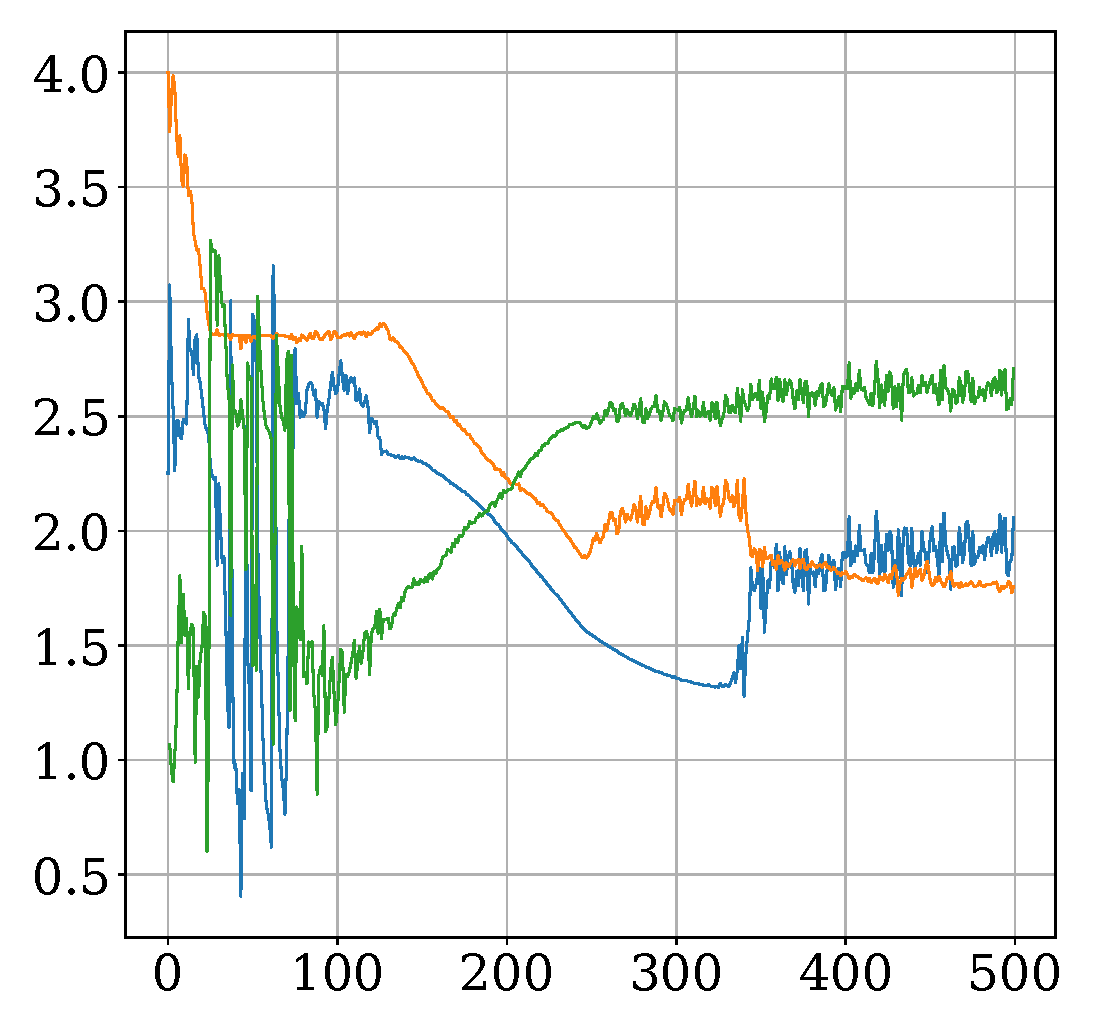
\includegraphics[width = 0.95\textwidth]{figures/912noise.eps}
\end{minipage}
\begin{minipage}{.32\textwidth}
\hspace{-3mm}
      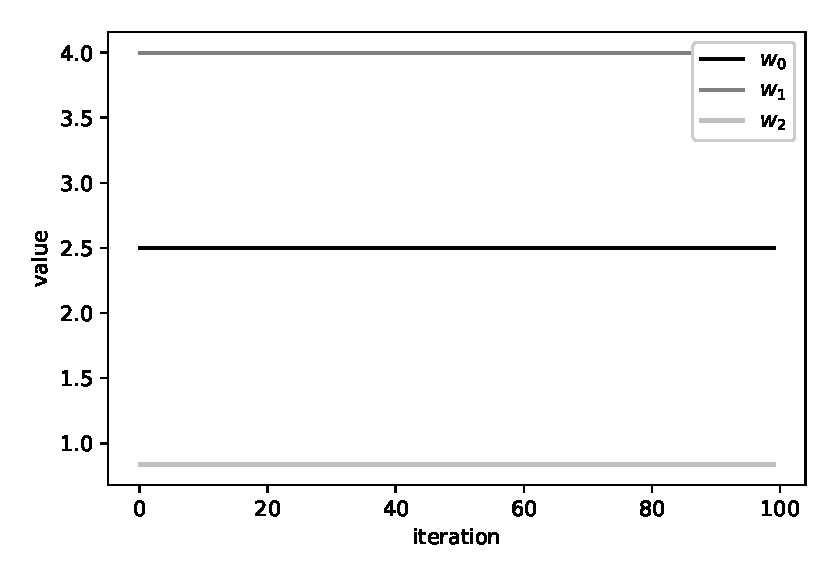
\includegraphics[width = 1.05\textwidth]{figures/900noise.eps}
\end{minipage}
\begin{minipage}{.32\textwidth}
\hspace{-2.1mm}
      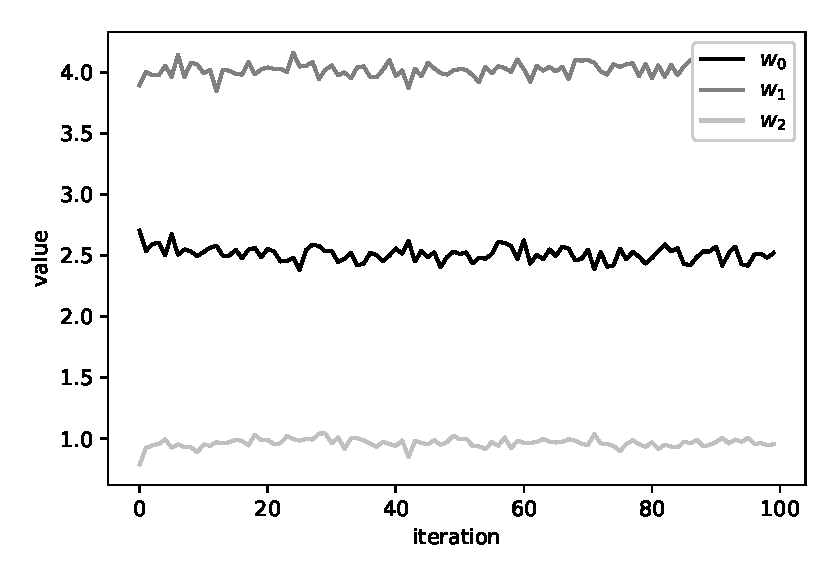
\includegraphics[width = \textwidth]{figures/901noise.eps}
\end{minipage}
\begin{minipage}{.32\textwidth}
\hspace{-2mm}
      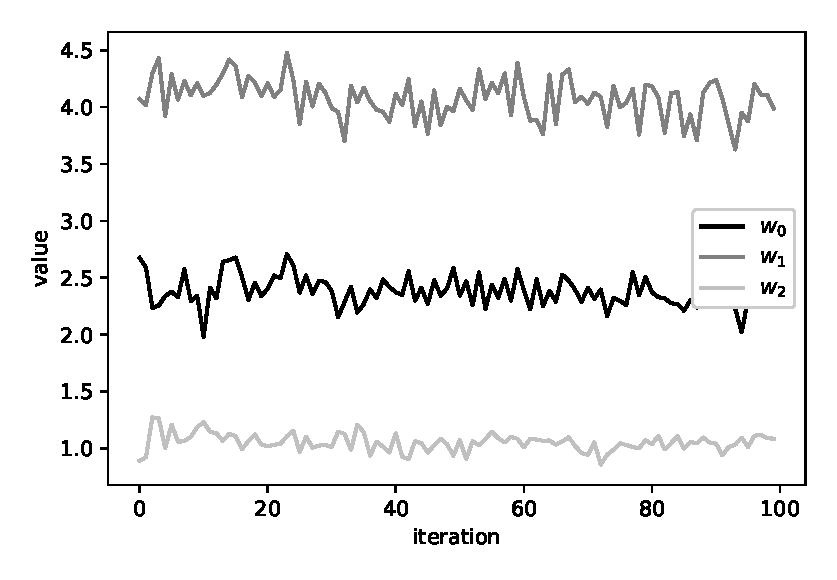
\includegraphics[width = 0.95\textwidth]{figures/902noise.eps}
\end{minipage}
\caption{Dependence of the parameters  $r$, $x_0$ and $y_0$ on the iteration number for different prior distributions. From top to bottom: plotting with a priori distribution; without specifying the prior distribution. From left to right: circumferences without noise; noise in the radius of the circle; noise in the radius of a circle as well as arbitrary points throughout the image.}
\label{ce:fig4}
\end{figure}

In this part of the experiment, an example of training a multi-model is shown to approximate several second-order figures simultaneously. A synthetic sample is used as data, which is obtained by generating three arbitrary non-intersecting circumferences, as well as adding noise to these circumferences. Noise was added to the radius of the circle for each point, and random points were added to the sample that do not belong to circumstances. The experiment compares two models: in the first model, the regularizer~$R\bigl(\mathbf {V}, \mathbf {W}, E(\Omega)\bigr) = 0,$ that is, the model without specifying the regularizer, in the second model regularizer:
\[
R\bigl(\mathbf{V}, \mathbf{W}, E(\Omega)\bigr)= -\sum_{k=1}^{K}\gamma\left(\mathbf{w}_k - \mathbf{w}_k^{0}\right)^{\mathsf{T}}\left(\mathbf{w}_k - \mathbf{w}_k^{0}\right),
\]
where~$\mathbf{w}_k^{0}$ a priori assumptions about the vector of parameters.

Figure~\ref{ce:fig3} shows the result of building an ensemble of locally approximating models that approximate the sample. Each local model approximates one circumference, and when adding different noise, the quality of the approximation will drop.
Figure~\ref{ce:fig4} shows a graph of the dependence of the radius of the circumferences $r$ and their centers $(x_0, y_0)$ on the iteration number. It can be seen that a model with a priori distribution converges faster than a model without a priori distribution.

\subsection{ Experiment with different noise levels and variance of the prior distribution }
\begin{figure}[h!t]\center
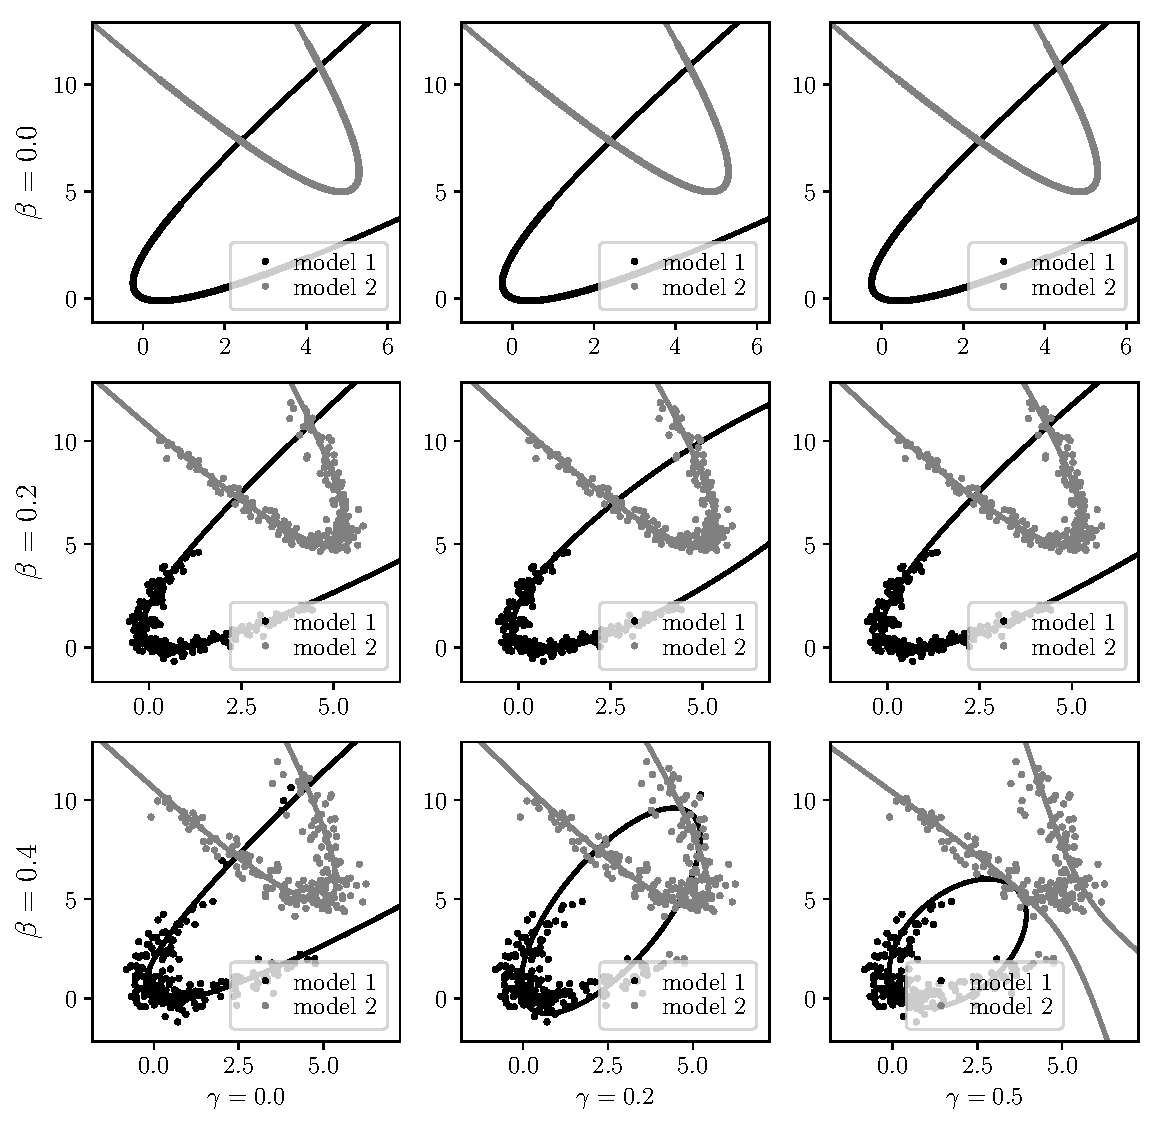
\includegraphics[width=0.8\textwidth]{figures/beta_gamma}
\caption{ The result of the approximation for data with different noise levels~$\beta$ and on the variance of the prior distribution~$\gamma$}
\label{ce:fig6}
\end{figure}

\begin{figure}[h!t]
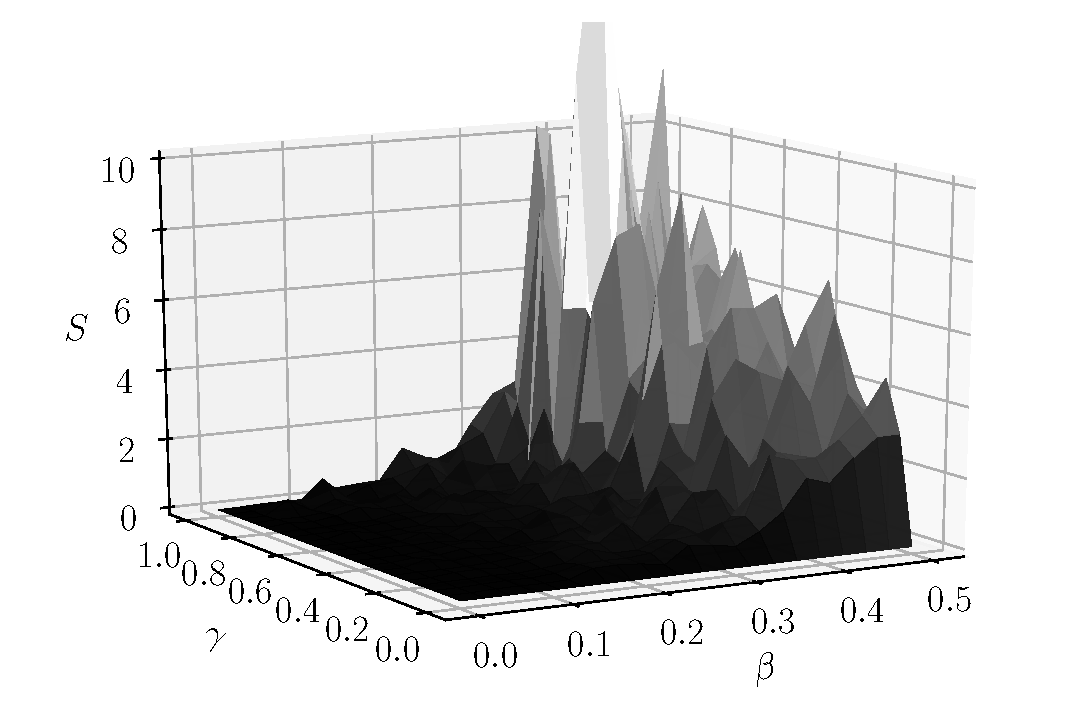
\includegraphics[width=0.5\textwidth]{figures/3dplot}
\caption{Dependence of models on the noise level~$\beta$ in the data, as well as on the variance of the prior distribution~$\gamma$}
\label{ce:fig5}
\end{figure}
In this part of the experiment, we analyze the quality of approximation~$S$ on the noise level~$\beta$ in the data and on the parameter of a priori distributions~$\gamma$. The sample is obtained as followsfirst, two vectors of parameters are randomly selected~$\mathbf{w}^\text{true}_{1}$ and~$\mathbf{w}^\text{true}_{2}$ are  coefficients of two parabolas. The vectors~$\mathbf {w}^\text {true}_{1} $ and~$\mathbf{w}^\text {true}_{2} $ are used to generate points~$x_i$ and~$y_i$ with normal noise added~$\varepsilon\sim\mathcal {N} \bigr(0,\beta\bigr)$. When training a multi-model, the prior distribution of parameters is considered~$\mathbf{w}_1\sim\mathcal{N}\bigr(\mathbf{w}^\text{true}_{1}, \gamma\mathbf{I}\bigr),\mathbf{w}_2\sim\mathcal{N}\bigr(\mathbf{w}^\text{true}_{2}, \gamma\mathbf{I}\bigr)$.

The following quality criterion is considered:
\[
S = ||\mathbf{w}^\text{pred}_{1} - \mathbf{w}^\text{true}_{1}||^{2}_{2} + ||\mathbf{w}^\text{pred}_{2} - \mathbf{w}^\text{true}_{2}||^{2}_{2},
\]
where~$\mathbf{w}^\text{pred}_{1}$ approximation of the vector of parameters of the first local model, and~$\mathbf{w}^\text{pred}_{2}$ approximation of the vector of parameters of the second local model.

Figure~\ref{ce:fig5} shows the dependence of the quality criterion~$S$ on the noise level~$\beta$ and the a priori distribution parameter~$\gamma$. The graph shows that at a low noise level~$\beta$ the quality of the approximation does not depend on the parameter~$\gamma $, and with an increase in the noise~$\beta $ the quality of the approximation~$S$ decreases.

Figure~\ref{ce:fig5} shows an example of how the algorithm works with different parameters~$\beta$ and $\gamma$. It is seen that in the absence of noise~$\beta$, both local models approximate the sample. With an increase in the noise level, the quality of the approximation decreases: at~$\beta = 0 {,}2$, with an increase in $\gamma$, the first local model from a parabola goes over to an ellipse; for~$\beta=0 {,}4$ as $\gamma$ increases, the first local model from a parabola goes over to an ellipse, and the second model from a parabola goes over to a hyperbola.

\subsection{Iris approximations }
\begin{figure}
     \centering
     \begin{subfigure}[b]{0.3\textwidth}
         \centering
         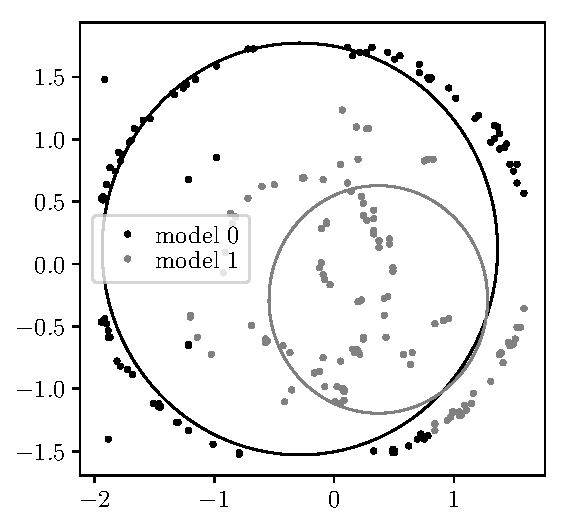
\includegraphics[width=\textwidth]{figures/not_prior_real_example}
         \caption{}
     \end{subfigure}
     \begin{subfigure}[b]{0.3\textwidth}
         \centering
         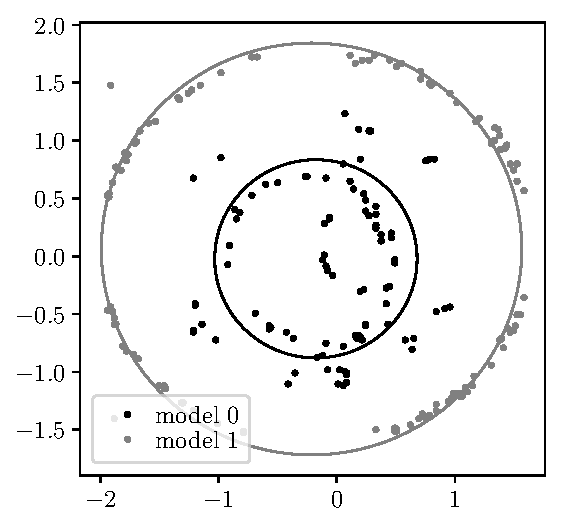
\includegraphics[width=\textwidth]{figures/prior_real_example}
         \caption{}
     \end{subfigure}
     \begin{subfigure}[b]{0.3\textwidth}
         \centering
         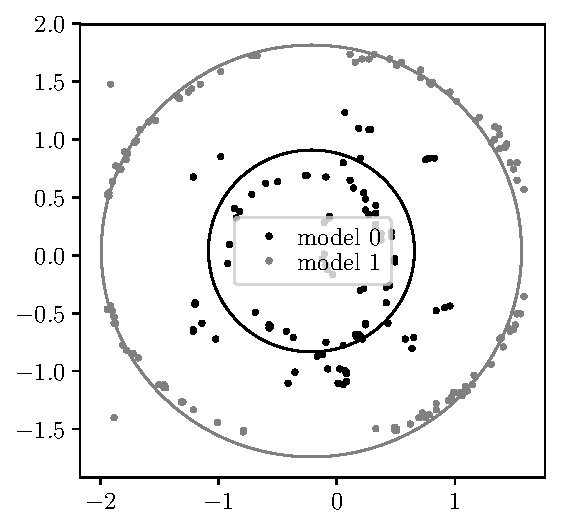
\includegraphics[width=\textwidth]{figures/prior_regular_real_example}
         \caption{}
     \end{subfigure}
     \caption{ Visualization of the approximation of the iris: a) if the $ R_0 $ regularizer is specified; b) if the $ R_1 $ regularizer is specified; b) if the $ R_2 $ regularizer is specified.}
    \label{ce:fig6}
\end{figure}

\begin{figure}
     \centering
     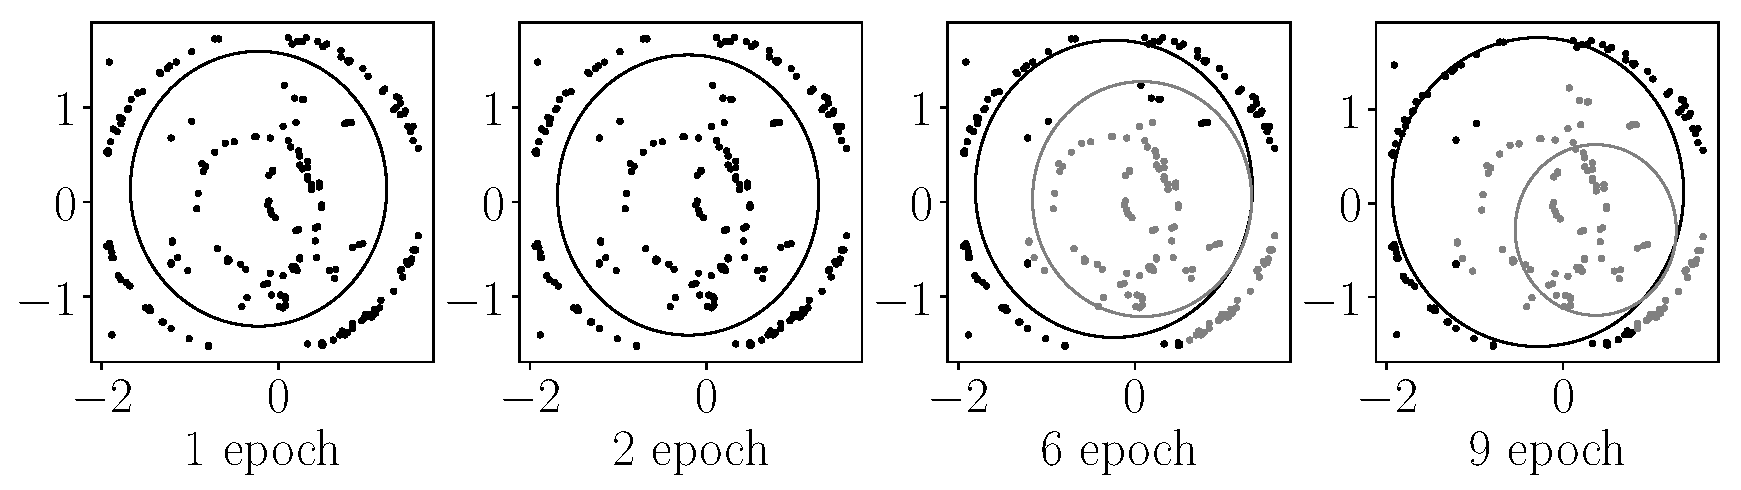
\includegraphics[width=\textwidth]{figures/experiment_real_not_prior}\\
     
     \caption{Visualization of the multi-model convergence process in the case of a regularizer~$R_0$}
    \label{ce:fig7}
\end{figure}

\begin{figure}
     \centering
     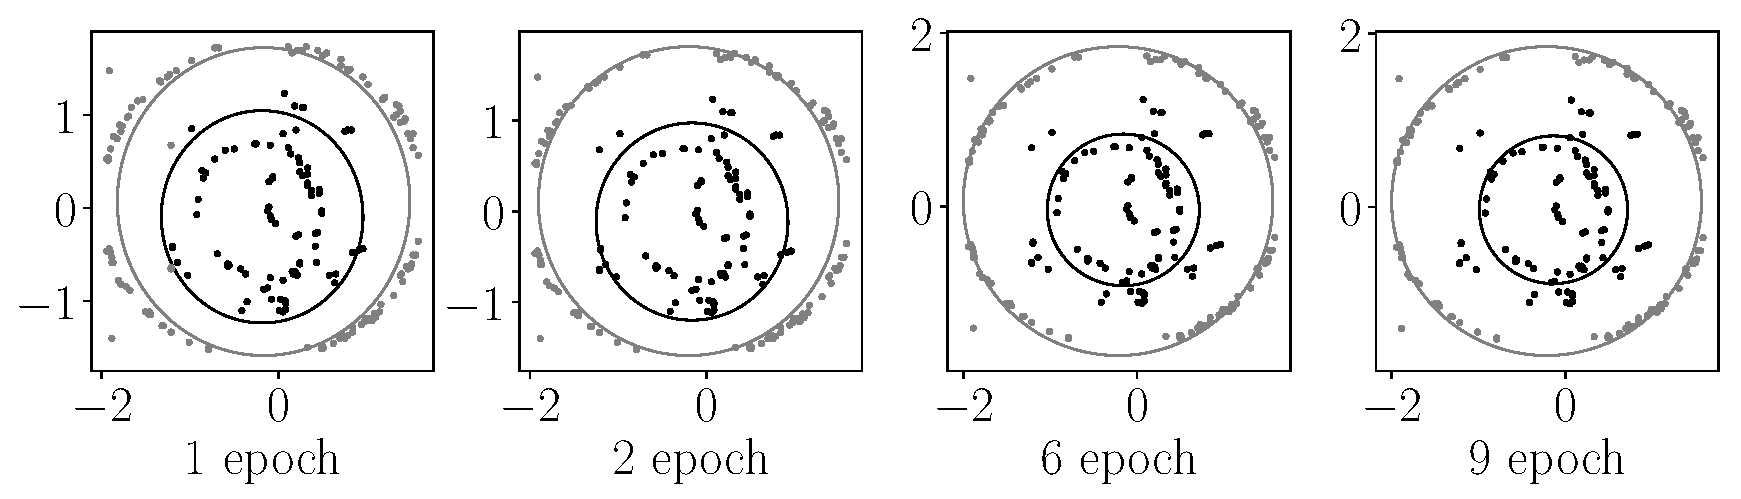
\includegraphics[width=\textwidth]{figures/experiment_real_prior}
     \caption{Visualization of the multi-model convergence process in the case of a regularizer~$R_1$}
    \label{ce:fig8}
\end{figure}

\begin{figure}
     \centering
     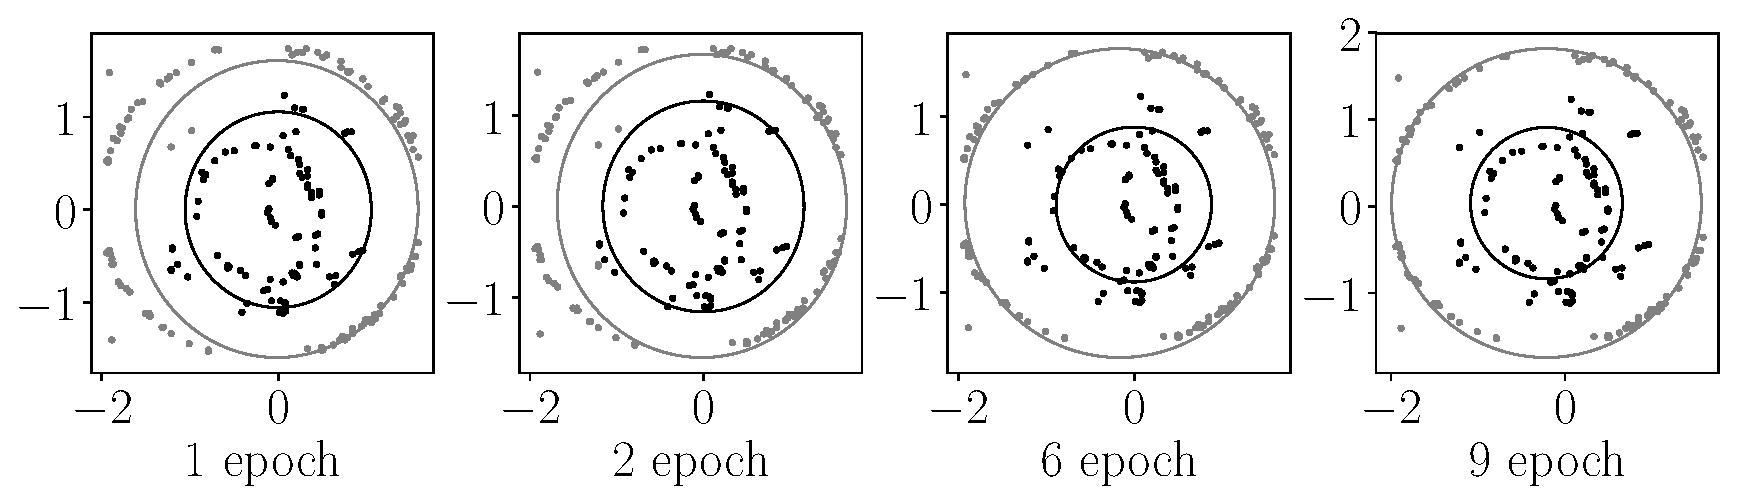
\includegraphics[width=\textwidth]{figures/experiment_real_regular}
     \caption{Visualization of the multi-model convergence process in the case of a regularizer~$R_2$}
    \label{ce:fig9}
\end{figure}

An analysis of the quality of the approximation is carried out for the problem of approximating the iris of the eye in the image. The iris of the eye consists of two concentric circumferences, therefore, a multi-model is considered, which consists of two experts: each expert approximates one of the circumstances. In a computational experiment, the quality of the approximation of circumferences is compared in the case of specifying different regularizers $R_0, R_1, R_2$. Regularizer$R_0\bigl(\mathbf{V}, \mathbf{W}, E(\Omega)\bigr)=0,$ that is, there is no regularizer. Regularizer:
\[
R_1\bigl(\mathbf{V}, \mathbf{W}, E(\Omega)\bigr)= -\sum_{k=1}^{K}\mathbf{w}_k^{\mathsf{T}}\mathbf{w}_k,
\]
which romotes near-zero parameters of local models.
Regularizer 
\[
R_2\bigl(\mathbf{V}, \mathbf{W}, E(\Omega)\bigr)= -\sum_{k=1}^{K}\mathbf{w}_k^{\mathsf{T}}\mathbf{w}_k + \sum_{k=1}^{K}\sum_{k'=1}^{K}\sum_{j=1}^2\left(w_k^j-w_k'^j\right)^2,\]
which promotes the coincidence of the centers of the circumferences and close to zero parameters of the model.
Figure~\ref{ce:fig6} shows the result of the eye iris approximation algorithm after 10 iterations. It can be seen that in the absence of a regularizer, one of the circumferences is found incorrectly. If the regularizer~$R_1 $ is given, the model approximates both circumferences with good quality, but the circumferences are not concentric. In case of specifying the regularizer~$R_2$, we get concentric circumferences on the image.

Figure~\ref{ce:fig7}--\ref{ce:fig9} shows the process of convergence of multi-models in the case of specifying different regularizers~$R_0, R_1, R_2$. It can be seen that the models with the regularizer type~$R_1$ and~$R_2$ approximate both circumferences, and the multi-model with the$R_0$ regularizer approximates only the large circumference.


\section{Conclusion}
The paper proposes a method for constructing interpretable machine learning models based on expert information. The problem of approximation of the second-order curves: parabola, hyperbola, ellipse is considered as a problem. Approximation of curves of the second order is applied in the problem of approximation of the iris of the eye.

An experiment was carried out during which the quality of the approximation of the second-order curves is analyzed depending on the initial noise level in the data, as well as depending on the regularizer. During the experiment, it was shown that with an increase in the noise level in the initial data, the approximation accuracy decreases: with a large noise, the shape of the approximated figure changes from a parabola to a hyperbola.
A computational experiment was carried out to approximate the iris of the eye using two concentric circles. The experiment shows that regularization based on expert information improves the quality of the approximation.

\begin{thebibliography}{99}
\bibitem{Ribeiro2016}
	\textit{Marco Tulio Ribeiro, Sameer Singh, Carlos Guestrin} "Why Should I Trust You?": Explaining the Predictions of Any Classifier // Proceedings of the 22nd ACM SIGKDD International Conference on Knowledge Discovery and Data Mining PP. 1135--1144. 2016

\bibitem{Tianqi2016}
	\textit{Chen Tianqi, Guestrin Carlos} XGBoost: A Scalable Tree Boosting System~// KDD ’16 Proceedings of the 22nd ACM SIGKDD International Conference on Knowledge Discovery and Data Mining. 2016.
	
\bibitem{Ishwaran2012}
	\textit{Chen Xi, Ishwaran Hemant} Random Forests for Genomic Data Analysis~// Genomics. 2012. Issues. 99, No 6. pp. 323--329.

\bibitem{Yuksel2012}
	\textit{Yuksel Seniha Esen, Wilson Joseph N., Gader Paul D} Twenty Years of Mixture of Experts~// IEEE Transactions on Neural Networks and Learning Systems. 2012. Issues. 23, No 8. pp. 1177--1193.


\bibitem{Cao2003}
	\textit{L.~Cao} Support vector machines experts for time series forecasting~// Neurocomputing, vol. 51, pp. 321–339, Apr. 2003.

\bibitem{Dempster1977}
	\textit{A. P. Dempster, N. M. Laird and D. B. Rubin} Maximum Likelihood from Incomplete Data via the EM Algorithm~// Journal of the Royal Statistical Society. Series B (Methodological), Vol. 39, No. 1 pp. 1-38, 1977.
	
	
\bibitem{Yumlu2003}
	\textit{M.\,S.~Yumlu, F.\,S.~Gurgen,  N.~Okay} Financial time series prediction using mixture of experts~// in Proc. 18th Int. Symp. Comput. Inf. Sci., 2003, pp. 553--560.
	
\bibitem{Cheung1995}
	\textit{Y.~M.~Cheung, W.~M.~Leung, and L. Xu} Application of mixture of experts model to financial time series forecasting~// in Proc. Int. Conf. Neural Netw. Signal Process., 1995, pp. 1--4.
	
\bibitem{Weigend2000}
	\textit{A. S. Weigend, S. Shi} Predicting daily probability distributions of S\&P500 returns~// J. Forecast., vol. 19, no. 4, pp. 375--392, 2000.
	
\bibitem{Ebrahimpour2009}
	\textit{R. Ebrahimpour, M. R. Moradian, A. Esmkhani, F. M. Jafarlou} Recognition of Persian handwritten digits using characterization loci and mixture of experts~// J. Digital Content Technol. Appl., vol. 3, no. 3, pp. 42–46, 2009.
	
\bibitem{Estabrooks2001}
	\textit{A.~Estabrooks, N.~Japkowicz} A mixture-of-experts framework for text classification~//in Proc. Workshop Comput. Natural Lang. Learn., Assoc. Comput. Linguist., 2001, pp. 1--8.
	
\bibitem{Mossavat2010}
	\textit{S. Mossavat, O. Amft, B. de Vries, P. Petkov, W. Kleijn} A Bayesian hierarchical mixture of experts approach to estimate speech quality~// in Proc. 2nd Int. Workshop Qual. Multimedia Exper., pp. 200--205., 2010
	
\bibitem{Sminchisescu2007}
	\textit{C. Sminchisescu, A. Kanaujia, and D. Metaxas} B M3 E: Discrimina- tive density propagation for visual tracking~// IEEE Trans. Pattern Anal. Mach. Intell., vol. 29, no. 11, pp. 2030–2044, 2007.
	
\bibitem{Matveev2010}
	\textit{I. Matveev} Detection of iris in image by interrelated maxima of brightness gradient projections~// Appl.Comput. Math. 9 (2), 252–257, 2010.

\bibitem{Matveev2014}
	\textit{I. Matveev, I. Simonenko}. Detecting precise iris boundaries by circular shortest path method~// Pattern Recognition and Image Analysis. 24. 304-309. 2014.
	
\bibitem{Bowyer2010}
	\textit{K. Bowyer, K. Hollingsworth, P. Flynn} A Survey of Iris Biometrics Research: 2008–2010.

\bibitem{Peng1996}
	\textit{F. Peng, R. A. Jacobs, M. A. Tanner} Bayesian inference in mixtures-of-experts and hierarchical mixtures-of-experts models with an application to speech recognition~// J. Amer. Stat. Assoc., vol. 91, no. 435, pp. 953–960, 1996.
	
\bibitem{Tuerk2001}
	\textit{A. Tuerk} The state based mixture of experts HMM with applications to the recognition of spontaneous speech~// Ph.D. thesis, Dept. Eng., Univ. Cambridge, Cambridge, U.K., 2001.
	
\bibitem{bishop2006}
	\textit{Bishop C.} Pattern Recognition and Machine Learning.~---~Berlin: Springer, 2006. 758~p.

\bibitem{Kaiming2015}
	\textit{Kaiming He} Deep Residual Learning for Image Recognition.
	
\bibitem{Han2020}
	\textit{Han Xu} Adversarial Attacks and Defenses in Images, Graphs and Text: A Review
	
\bibitem{Xingjun2019}
	\textit{Xingjun Ma} Understanding Adversarial Attacks on Deep Learning Based Medical Image Analysis Systems
	
\bibitem{Akhtar2018}
	\textit{Naveed Akhtar} Threat of Adversarial Attacks on Deep Learning in Computer Vision: A Survey
	
\bibitem{Dalila2018}
	\textit{Salamani Dalila} Deep generative models for fast shower simulation in ATLAS
	
 \end{thebibliography}


\end{document}

